
The remote sensing of any atmospheric component is based on its interaction with
electromagnetic radiation. By inverting this interaction, the measured radiation
can be used to infer certain properties of that component. This chapter presents
the physical processes, which enable satellites to sense clouds and
precipitation as well as the practical aspects of observing the
atmosphere from space.


The first part of this chapter provides a brief introduction to
radiative transfer (RT) theory, which can be used to describe  the
interaction of radiation with the atmosphere. Based on this, the
principal characteristics of observations across the electromagnetic
spectrum and their sensitivity to hydrometeors%
\footnote{%
Hydrometeor is the collective term for the liquid and frozen particles that
that make up clouds and precipitation.
}%
 are discussed. The remaining part of this chapter then provides an overview of
 the types of satellite observations that were used in the retrieval
 applications that were developed as part of this thesis.
The presentation focuses on observations measuring radiation that is
emitted from the sun or the Earth and its atmosphere, so called
\textit{passive observations}.
%to the electromagnetic radiation measured by satellites. This is
%followed by a discussion of the different types of satellite observations
%relevant to this thesis and their characteristics.


%Doing so, requires a quantitative model of the propagation of radiation through
%the atmosphere. Such a model is provided by the physical theory of 
%Since radiative transfer theory is fundamental to atmospheric remote sensing ,
%this section provides an introduction to radiative transfer in the atmosphere.
%The focus is put on the interaction of radiation with hydrometeors. This
%presentation is mostly based on the more comprehensive texts by Mishchenko et
%al. (2002), Thomas and Stamnes (2002), and Wallace and Hobbs (2006).


\section{Radiative transfer theory}

Radiative transfer theory describes the propagation of a perfectly monochromatic
beam of light through a medium. As this beam propagates through the medium it
interacts with it through electromagnetic and quantum mechanical processes.
Radiative transfer theory provides a simplified model of these interactions,
which is well suited for the conditions of passive remote sensing of the
atmosphere.  The following presentation is  based on the more
comprehensive texts by \citet{mishenko02}, \citet{thomas02} and \citet{wallace06}.
%al. (2002), Thomas and Stamnes (2002), and Wallace and Hobbs (2006).

Electromagnetic sensors measure the mean total energy that is transferred by
electromagnetic radiation over a finite time interval. The way in which this
energy is distributed across the components of the electric field is defined as
its \textit{polarization state}. Mathematically, the polarization state of the
beam can be described using the four dimensional Stokes vector
\begin{align}
  \bm{I} &= \left [ \begin{array}{c}
    I \\
    Q \\
    U \\
    V \\
    \end{array} \right ]
\end{align}
The components $I, Q, U$ and $V$ are called the Stokes parameters and have the
unit of monochromatic energy flux per solid angle. The Stokes vector fully
describes the state of a monochromatic beam of radiation to the extent that it
can be measured by an electromagnetic sensor. Thus any electromagnetic
measurement can be derived from knowledge of the Stokes vector at the position
and orientation of the sensor. Radiative transfer theory describes how the
Stokes vector changes as it propagates through a medium.

\subsection{Interactions with matter}

Radiative transfer theory distinguishes three fundamental processes through
which matter interacts with radiation. These are the emission of
electromagnetic radiation, its absorption and scattering.

\subsubsection{Emission}

At temperatures above absolute zero, all matter emits thermal radiation. Thermal
radiation is produced when matter transitions from a quantum mechanical state
of higher energy to one of lower energy causing the excess energy to be emitted
in the form of radiation. The amount of radiation of a given frequency $\nu$
emitted by a body depends on its temperature and material. It is typically
modeled using a material-dependent emissivity vector $\vec{e}$, which relates
the emission of the material to that of an ideal black body, i. e. a material
that absorbs all incoming radiation:
 \begin{align}
   \label{eq:emissivity}
   \vec{I} &= (\vec{e} \cdot ds) B(T, \nu)
 \end{align}
 Here $B(T, \nu)$ is the radiation emitted by a black body at temperature $T$
 and frequency $\nu$, which is described by Planck's law
 \begin{align}
   B(T, \nu) &= \frac{2 \nu^2}{c^2}\frac{h\nu}{e^{\frac{h\nu}{k T}} - 1},
 \end{align}
 with $c$ is the speed of light in vacuum, $h$  the Planck constant and $k$
 the Boltzmann constant.

 The emissivity is a material property of the medium through which the beam
 propagates and depends on its quantum mechanical properties as well as the
 wavelength of the radiation. The emissivity vector defined above is a
 differential quantity that describes emission from a volume element along an
 infinitesimal step of the propagation path of the beam.


%For a material that is opaque, there is no need to integrate over the full
%volume, since only its surface will contribute to the observed emission.
%The emissivity of a surface can be described using an emissivity vector
%$\vec{e}$ in the same way as for emission from a volume, with the difference
%that its components are unitless and integration over the propagation path is
%not required.

\subsubsection{Absorption}

Absorption refers to the process of radiation being converted into internal
energy of the matter it interacts with. Mathematically, this process is
described by the absorption vector $\vec{\alpha}$, defined as the fraction of
the incoming radiation that is absorbed along an infinitesimal distance $ds$
along the propagation path:
\begin{align}
\vec{I}_\text{absorbed} &= (\vec{\alpha} \cdot\ ds) \odot \vec{I}
\end{align}
Here $\odot$ denotes the element-wise product of the absorption vector and
the Stokes vector $\vec{I}$ of the incoming radiation. Absorption may be
understood as the inverse process of thermal emission. Formally, this is
expressed by Kirhoff's  law of radiation
\begin{align}
  \vec{\alpha} &= \vec{\epsilon},
\end{align}
which states that the absorption vector is identical to the emissivity vector
defined in Eq.~\ref{eq:emissivity}. This law is applicable to all matter in the
atmosphere given that it is in a state of local thermal equilibrium (LTE). LTE
occurs when the density of matter is sufficiently high so that the population
rates of energy states above the ground state are determined by thermal
collisions rather than the absorption of radiation. This decouples the emission
of radiation from the radiation field itself, allowing the simplified treatment
of matter as thermal emitters with the emission rates independent of the
radiation field. LTE is a valid assumption for radiative transfer in the
troposphere.

\subsubsection{Scattering}

Scattering describes the effect that inhomogeneities of the medium have on the
propagation of the beam. When a plane-parallel electromagnetic wave encounters
such inhomogeneities, it is scattered in all directions. Mathematically, the
scattering of a beam of light propagating in direction $\vec{n}$ into the
direction $\vec{\hat{n}}$ is described by the phase matrix
$\mat{Z}(\vec{\hat{n}}, \vec{n})$:
\begin{align}
  \vec{I}_\text{scattered}(\vec{\hat{n}}) &= \mat{Z}(\vec{\hat{n}}, \vec{n}) \vec{I}(\vec{n})
\end{align}
Since parts of the energy flux of the beam are deviated from the direction of
propagation, the intensity of the radiation along the beam is decreased. As it
propagates through the medium, the intensity of a beam is thus decreased by the
effects of absorption and scattering. The combination of these two processes is
referred to as \textit{attenuation} or \textit{extinction} and is described by
the attenuation matrix $\mat{K}$, which is the sum of the absorption vector
$\vec{\alpha}$ and the fraction of radiation scattered away from the propagation
path:
\newcommand*{\vertbar}{\rule[-1ex]{0.5pt}{2.5ex}}
\newcommand*{\horzbar}{\rule[.5ex]{2.5ex}{0.5pt}}
\begin{align}
  \vec{K} &=
  \left [ \begin{array}{cccc}
      \vertbar & \vertbar & \vertbar & \vertbar \\
      \vec{\alpha} & \vec{0} & \vec{0} & \vec{0} \\
      \vertbar & \vertbar & \vertbar & \vertbar
    \end{array} \right ]
       + \int_{\vec{\hat{n}}} d\vec{\hat{n}}\ \mat{Z}(\vec{\hat{n}}, \vec{n})
\end{align}

The strength of the scattering interaction depends on the relation of the size
of the inhomogeneities and the wavelength of the radiation. When the scale of
inhomogeneities is much smaller than the wavelength, the effects of scattering
can often be neglected. As the size of the inhomogeneities increases, the
strengths of the scattering increases and scattering effects must be taken into
account. The scattering interaction drastically complicates calculating the
evolution of the radiation because it requires taking into account the radiation
that is scattered into the line of sight from all directions. Because of their
relatively large size, scattering effects of hydrometeors need to be taken into
account across most of the electromagnetic spectrum. Simulations of radiative
transfer that involve hydrometeors are therefore more complex to perform than
those that don't.


\subsection{The radiative transfer equation}

The previous section introduced the fundamental interactions of radiation
with matter and how they are described mathematically in radiative transfer
theory. Combining the three processes of emission, absorption and scattering,
the change that a beam undergoes as it travels a distance $ds$ along its
propagation path through the atmosphere is described the vector radiative
transfer equation (VRTE):
\begin{align}\label{eq:vrte}
  \frac{d\vec{I}(\vec{n})}{ds} &=
  -\mat{K}\vec{I}(\vec{n}) + \vec{\alpha} \cdot B_\nu(T) + \int_{\hat{\vec{n}}} d\hat{\vec{n}} \ \mathbf{Z}(\vec{n}, \vec{\hat{n}}) \vec{I}(\vec{\hat{n}}).
  \end{align}

The first term on the right hand side is the extinction term, which represents
the combined effects of absorption and scattering of radiation out of the
propagation direction, which act to decrease the intensity of the radiation
along the line of sight. The second term represents emission along the line of
propagation, with the emissivity vector $\bm{\epsilon}$ replaced by the
absorption vector $\bm{a}$ according to Kirchoff's law of thermal radiation.
The third term represents the radiation that is scattered into the line of
sight. Both of these terms act to increase the intensity of the beam. 

\section{Observations of hydrometeors}
%
\begin{figure}[!tbp]
  \centering
  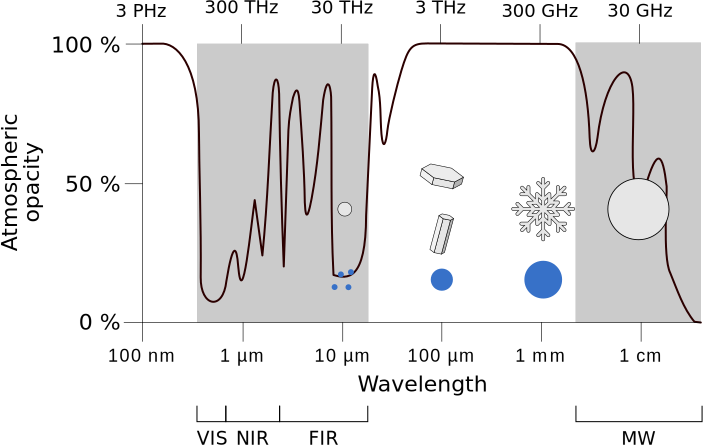
\includegraphics[width=0.75\textwidth]{spectrum}
  \caption{Overview of the electromagnetic spectrum used for hydrometeor retrievals. The black
    curve shows the variation of the atmospheric opacity across the spectrum.}
  \label{fig:radiative_transfer:spectrum}
\end{figure}

Radiative transfer theory describes the propagation of radiation through the
atmosphere in terms of its radiative properties, which are represented by the
absorption vector $\vec{\alpha}$, the extinction matrix $\vec{K}$ and the phase
matrix $\vec{Z}$. In order to apply radiative transfer theory to gain an
understanding of remote sensing observations of the atmosphere, the gases,
aerosols and hydrometeors contained in it must be related to its radiative
properties.

The radiative properties of the atmosphere are strongly dependent on the
wavelength $\lambda$ at which it is observed. The applications presented in this
thesis focus on observations from the visible (VIS,
$\SI{350}{\nano \meter} \leq \lambda < \SI{720}{\nano \meter}$), infrared (IR,
$\SI{0.72}{\micro \meter} \leq \lambda < \SI{20}{\micro \meter}$), and microwave
(MW, $\SI{1}{\milli \meter} \leq \lambda < \SI{1}{\meter}$) regions, which
encompass most commonly used wavelength for the remote sensing of clouds and
precipitation.

An overview these regions within spectrum of electromagnetic radiation is
provided in Fig.~\ref{fig:radiative_transfer:spectrum}. The graph provides an
approximate depiction of the atmospheric opacity in the absence of hydrometeors.
When viewed from a satellite, the atmospheric opacity gives an indication of how
far down into the atmosphere a sensor can 'see'. Generally, where the opacity is
low, the satellite can see down to the surface, while where it is high it is
sensitive only to the upper parts of the atmosphere.

Observations of the atmosphere are the results of the combined effects of gases,
aerosols and hydrometeors in the atmosphere. To gain an understanding of the
information that certain observations provide on hydrometeors, it is helpful to
decompose the contributions into a clear-sky component, which takes into account
only the effects of molecules aerosols, and a cloudy-sky component, which takes
into account the effects of hydrometeors. As a first approximation, the clear-sky
component maybe viewed as the background upon which the hydrometeors are
observed.

\subsection{The atmospheric background}

Observations at short wavelengths differ from those at long wavelengths with
respect the source of the observed radiation. At wavelengths in the visible and
near infrared regions, the largest part of the observed radiation stems from the
sun. This is because, at these short wavelengths, black body radiation at
typical atmospheric temperatures is small compared to reflection of solar
radiation. As the wavelength increases, the intensity of solar radiation decreases
while that of a black bodies at atmospheric temperatures increases. At wavelengths
exceeding $\approx \SI{3}{\micro \meter}$, emission from atmospheric constituents
dominates the intensity of reflected solar radiation. This threshold separates
the thermal ($\lambda \geq \SI{3}{\micro \meter}$) from the near infrared. At
these wavelengths solar emission can generally be neglected and all observed
radiation originates from the atmosphere itself or the Earth's surface.

The atmospheric opacity displayed in Fig.~\ref{fig:radiative_transfer:spectrum}
corresponds to the combined effects of absorption and extinction by gases in the
atmosphere. Gases affect radiation mostly through absorption and emission, while
scattering plays a role only in the visible range. The reason for this is the
small size of the molecules (around $\SI{1}{\nano \meter}$) compared to the
wavelengths of the radiation.

There is little absorption in the visible range with most of it due to water
vapor. In the near and thermal infrared, absorption increases but is concentrated
in discrete absorption bands, which makes the opacity of atmosphere highly
variable across wavelengths. The principal gaseous absorbers in the infrared
region are water vapor, cabon dioxide and ozone. Absorption also plays an
important role in the microwave region with significant contributions from water
vapor, oxygen, nitrogen and ozone. 

In addition to the effects of gases, satellite observations can be affected by
the presence of aerosols. Aerosols are larger than gas molecules but their
scattering and absorption effects remain mostly limited to the VIS and NIR
regions. At longer wavelength, aerosols have no significant effect on the
observations.

\subsection{Physical and radiative properties of hydrometeors}

The radiative properties of hydrometeors depend on their size and whether they
are in the liquid or frozen phase. Because the dielectric properties of ice and
water differ significantly across the electromagnetic spectrum, hydrometeors of
similar sizes have drastically different radiative properties in certain
wavelength domains. To provide an overview of the sizes of the principal classes
of hydrometeors with respect to the wavelengths of the electromagnetic spectrum,
they are displayed in Fig.~\ref{fig:radiative_transfer:spectrum} at the
wavelengths corresponding to their approximate sizes. Liquid hydrometeors are
identified using blue coloring, while white corresponds to frozen hydrometeors.

Among the smallest hydrometeors are liquid cloud droplets with typical sizes
around $\SI{5}{\micro \meter}$. At sizes of around $\SI{25}{\micro \meter}$,
water drops become large enough to fall out of the clouds. Small, precipitating
liquid droplets that range in size from $25 to \SI{250}{\micro \meter}$ are
referred to as drizzle. Larger drops are classified as rain. Typical sizes of
rain drops are around $\SI{1}{\milli \meter}$ but can become as large as
$\SI{5}{\milli \meter}$.

At temperatures below $\SI{0}{\celsius}$ ice crystals can form in the
atmosphere. Their sizes range from $\SI{1}{\micro \meter}$ to
$\SI{1.5}{\milli \meter}$ with typical sizes around $\SI{100}{\micro \meter}$.
Snow flakes are aggregates, which form through the collision of ice crystals.
These range in size from hundreds of micrometers millimeters to several
centimeters.

When snowflakes collide with liquid drops at temperatures below
$\SI{0}{\celsius}$, the liquid drop freezes upon the snowflake causing it to
grow. This process is called riming. Heavily rimed snowflakes are referred to as
graupel and have typical sizes of around $\SI{1}{\centi \meter}$. Finally, the
largest hydrometeors are hailstones, which form only in strong thunderstorms and
can reach sizes of up to $\SI{10}{\centi \meter}$$.


%Most observations of clouds are affected not only by the clouds themselves but
%also by other constituents of the atmosphere. In the following, we will
%therefore first discuss observations without clouds, so called \textit{clear
%  sky} observations, as these form the background for the observations of
%hydrometeors. This is followed by a discussion of the observable effects of
%hydrometeors on the observations, which gives rise to the signal in the
%\textit{all-sky observations} that can be used to infer the physical properties
%of hydrometeors.

%\subsection{The Earth's surface}
%
%The characteristics of the Earth's surface vary considerably across the
%electromagnetic spectrum. In the visible range, the surface absorbs large parts
%of the radation. The darkest surfaces are the ocean which absorbs around
%$\SI{95}{\percent}$ of the incoming radiation. Bare land surface and forests are
%considerable brighter but still absorb most ($\approx \SI{75}{\percent}$) of the
%incoming radiation. In contrast to that, snow and ice covered surface reflect
%nearly all of the incoming radiation and thus appear very bright.
%
%In the infrared region of the electromagnetic spectrum the emissivity of the Earth surface
%increases significantly. For wavelengths between $3$ and $\SI{20}{\micro \meter}$ the emissivity
%of most surface types is larger than $0.9$. At these wavelengths the surface is very effective at
%emitting and absorbing radiation and there is little contrast between different surface types.
%
%In the microwave region surface emissivity patterns are more complex. Emissivity
%from land is relatively high, while emissivity from water surfaces is low. The
%contrast between land and surface increases with the wavelength. Emissivities
%from snow and ice are lower than that of most bare land surface but higher than
%that of water. The emissivity furthermore depends on the viewing angle and the
%polarization of the radiation.
%
%While these general tendencies are helpful for a qualitative analysis of
%satellite imagery, it should be noted that they only provide a rough
%characterization of the behavior of the Earth's surface across the
%electromagnetic spectrum. Accurate, quantitative modeling of surface
%emissivities is still an unsolved problem and thus remains an area of
%active research.

\subsection{Cloudy sky}

Due to their comparably large sizes, the scattering effects of hydrometeors need
to be taken into account across most wavelengths from the VIS to the MW regions.
In the VIS and NIR there is little absorption from either water or ice.
Hydrometeors thus mostly deviate radiation from its propagation path without
significantly decreasing its intensity. Clouds observed at these wavelengths
typically appear bright because the solar radiation scattered back towards
the sensor is much more intense than reflection from the surface.

In the FIR region, both water and ice are strongly absorbing. Because the
ambient temperature decreases with altitude in the troposphere, opaque clouds
emit less intense radiation than the surface or water vapor below them.
At wavelength at which there is weak absorption from water vapor, so called
\textit{window channels}, radiation from opaque clouds can be used to
infer the temperature at the cloud top, which is related to the altitude of
the cloud.

At microwave frequencies, liquid water is a much more efficient absorber than
ice. Furthermore, for passive observations the scattering from hydrometeors at
frequencies below $\SI{50}{\giga \hertz}$ can be neglected. The principal
interaction with hydrometeors at these wavelength is therefore thermal emission
and absorption from liquid cloud droplets and precipitation. Since water
surfaces have low emissivities at these wavelengths, emission from liquid
hydrometeors causes a distinct signal in the observations.

At frequencies above $\SI{50}{\giga \hertz}$, passive microwave observations
become sensitive to the scattering from large snow flakes. This scattering
signal is important for sensing precipitation over land, where the emission
signature from liquid hydrometeors may not be detectable due to the much warmer
background surface.

\section{Satellite observations}

The information content of satellite observations on hydrometeors is strongly
dependent on the wavelength of the radiation. Because radiation at different
wavelengths is sensitive to different properties and types of hydrometeors, 
observations at different wavelength provide complementary information on
them. In addition to the wavelength, other characteristics of the observations
such as temporal and spatial resolution determine how well different satellite
observations can be used to characterize hydrometeors from space.

Due to the technical complexity of operating specialized sensors in space, the
availability of observations and their characteristics are ultimately determined
by a trade-off between technical and financial constraints on the one side and
scientific value on the other. Since there is only a very limited number of
satellite mission dedicated specifically to observations of hydrometeors,
leveraging the full potential of available satellite imagery requires exploiting
and combining a wide range of observations of different types.

\subsection{Sensor types}

The above discussion of radiative transfer in the atmosphere focused on
observations of radiation that originates either from the sun or the Earth and
its atmosphere. Sensors that measure these types of radiation are called passive
sensors because they do not emit any radiation themselves. \textit{Active
sensors}, on the other hand, emit radiation and measure how much of that
radiation is scattered back to the sensor. The active sensors that are used for
the remote sensing of hydrometeors are mainly radars and lidars. These sensors
measure the time of travel between emission and reflection, which can be used to
infer the distance from the detector in addition to the intensity of the
reflected radiation. This allows them to profile the atmosphere along the line
of sight, leading to much higher vertical resolution than what can be obtained
with passive sensors.

From an observational perspective, the principal difference between radars and
lidars are the wavelengths at which they operate. Lidars employ radiation with
relatively short wavelengths, which makes them sensitive to very small
hydrometeors as well as molecules and aerosols in the atmosphere. In contrast to
that, radars operate at MW wavelengths, which makes the sensitive only to
hydrometeors. In general, active sensors are much more sensitive to the
scattering from small particles than their passive counterparts because of the
intensity of the emitted beam.

\subsection{Resolution and coverage}

In addition to the information content that observations can provide on
hydrometeors, their ability to resolve spatial and temporal variability as well
as how much of the globe they cover are important characteristics, which
influence their suitability for different applications.

The orbit in which a satellite is placed plays an important role in determining
these characteristics. For earth observations, two principal classes of orbits
can be distinguished: Geostationary and low-earth orbits. Satellites in
geostationary orbit rotate around the Earth at the same angular velocity as the
Earth rotates around its axis. This allows them to hover over the same position
on the Earth's surface. Since the field of view of the satellite is constant it
can provide observations with high temporal resolution at all locations below
the satellite. This makes these satellite suitable for many near real-time
applications in weather forecasting.

The disadvantage of geostationary platforms is their long distance from the
Earth, which is around $36\ \SI{000}{\kilo \meter}$. Since the spatial
resolution of microwave sensors is limited by the long wavelengths of the
radiation, they are currently not deployed on these platforms. Geostationary
therefore typically carry VIS and IR sensors, which can produce observations
at very high spatial resolutions. Besides that, geostationary satellites
are always located over or close to the locator. The resulting viewing geometry
causes their resolution to degrade at high latitudes.

A common type of low-Earth orbit used for Earth observing satellites are polar
orbits in which the satellite passes above or nearly above the poles. The
rotation of the Earth between consecutive orbits allows these satellites to
achieve global coverage. The low altitude of these orbits ($300
- \SI{1000}{\kilo \meter}$) makes them suitable also for microwave sensors but
decreases the spatial coverage of the sensor. The swaths of sensors in low-earth
orbits are typically limited to a few thousand kilometers in width. Depending on
the exact size of the field of view and the location on Earth, the time between
consecutive overpasses for a fixed position can be as high as $\SI{12}{\hour}.

Fig.~\ref{fig:remote_sensing:viewing_geometries} shows the field of views of
the Advanced Baseline Imager on the GOES 16 geostationary satellite and the
GPM Microwave Imager on the polar-orbiting GPM Core Observatory. The observations
from both satellites are projected onto the corresponding location on the Earth.
This illustration clearly shows the differences that the satellite orbit makes
for the observations. While the geostationary satellite can permanently observe
a large part of the hemisphere below it, the polar orbiting satellite sees only
a comparably thin stripe of the globe.

\begin{figure}[!hbpt]
  \centering
  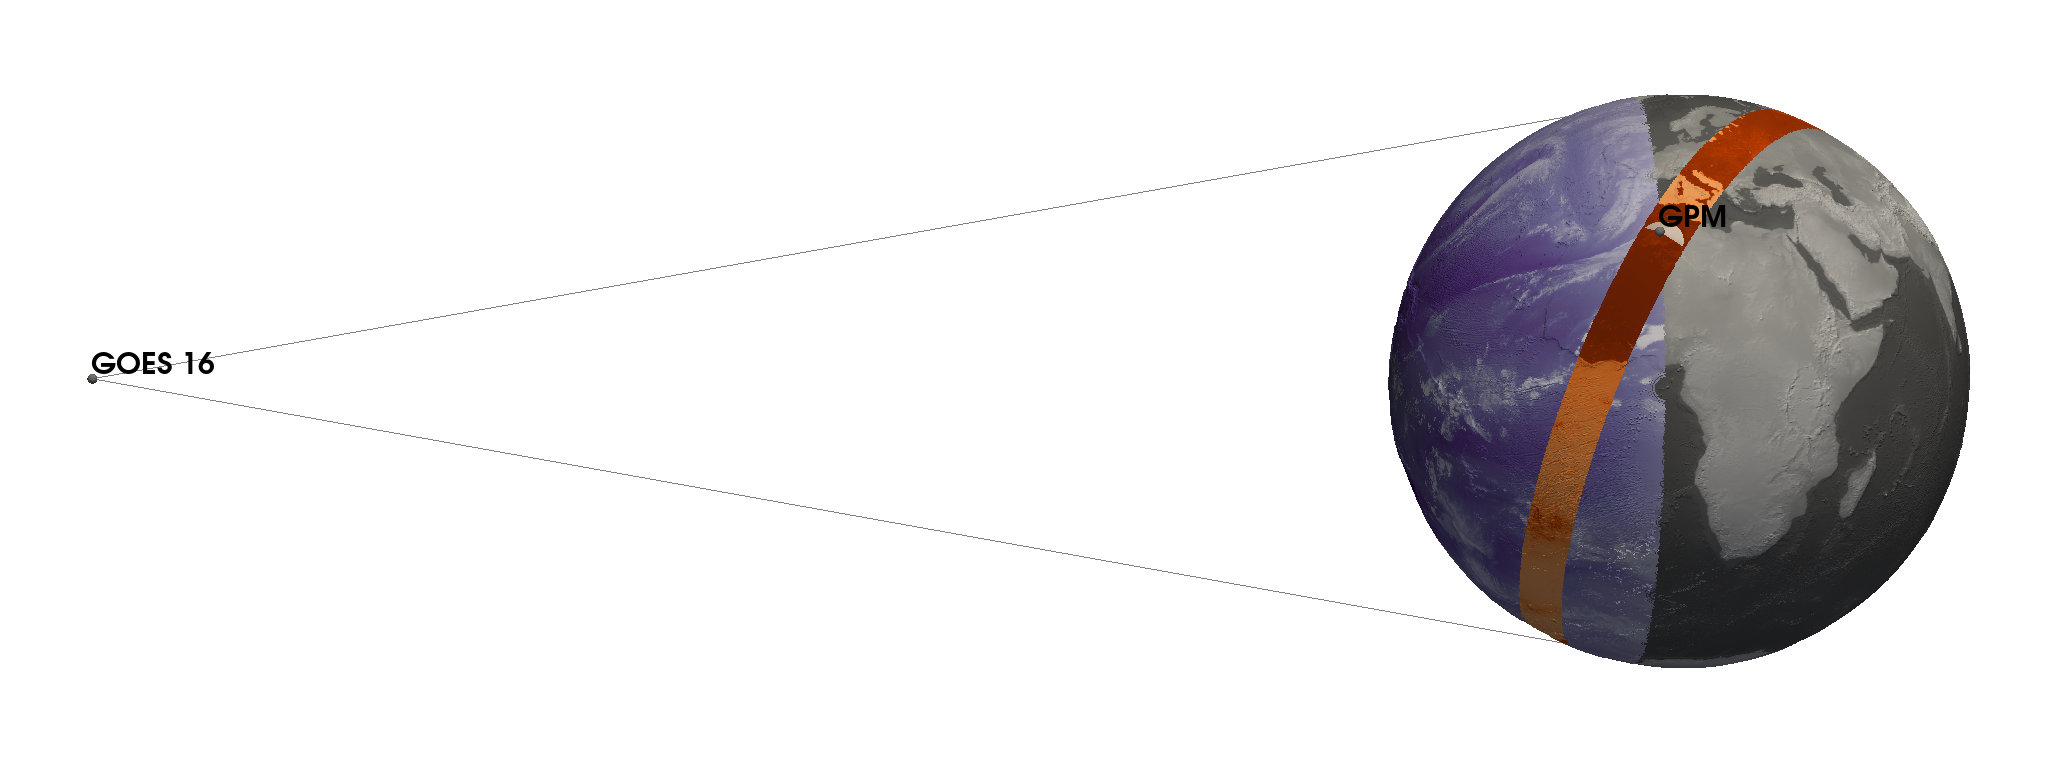
\includegraphics[width=0.8\textwidth]{viewing_geometries}
  \caption{Viewing geometries of geostationary and polar-orbiting satellites
  drawn to scale. The illustration shows geo-located satellite observations from
  the GOES 16 geostationary satellite in purple and from the polar-orbiting GPM
  Core Observatory in orange. The black spheres mark the instantaneous satellite
  positions.}
  \label{fig:remote_sensing:viewing_geometries}
\end{figure}

\subsection{Example: Satllite observations of Hurricane Ida}

Figure~\ref{fig:radiative_transfer:observations} illustrates the different types
of observations used for the remote sensing of hydrometeors using observations
of Hurricane Ida shortly before landfall on August 30, 2021. The first row of
panels shows observations derived from the Advanced Baseline Imager on the GOES
16 geostationary satellite. Panel (a) shows a natural color composite, which
combines observations from 3 channels from the VIS and NIR to create an image
emulating human color vision. Panel (b) shows observations from the NIR.
Differences in the dielectric constant of water and ice cause ice clouds to
absorb incoming solar radiation much more strongly than water clouds. The high
ice clouds that cover the Hurricane therefore appear much darker than in the RGB
image. Panel (c) shows observation from a window channel in the FIR. Since it is
a window channel, most of the radiation observed in cloud free areas stems from
the Earth's surface and thus appear bright. Where clouds are present the
observed brightness temperatures are closely related to the atmospheric
temperature at the altitude of the cloud and thus colder than the surface.

Panel (c) and (d) show passive microwave observations at $\SI{18.7}{\giga
  \hertz}$ and $\SI{166}{\giga \hertz}$. At the very low microwave frequencies
only the a thermal emission from precipitation in the hurricane is visible over
the cold ocean surface, while the clouds overland yield no signal. At the higher
microwave frequencies, the surface is not visible due to emission from water
vapor. Scattering by snow particles causes a cold scattering signal from the
thickest clouds around the Hurricane.

Finally, panel (e) shows Ku-band radar reflectivities from the GPM
dual-frequency precipitation radar along a vertical cross section of the
Hurricane. The signal in the radar observations is the amount of energy that is
reflected back to the sensor. Due to the relatively low frequency of the
radar, it is only sensitive to large, precipitation hydrometeors.


\begin{figure}
  \centering
\includegraphics[width=\textwidth]{observations}
\caption{Satellite observations of Hurricane Ida on 2021-08-29 15:09 UTC.
  Panels (a), (b), (c) show observations from the VIS and IR regions obtained
  by the Advanced Baseline Imager on the GOES 16 geostarionary satellite.
  Panels (d) and (e) show passive microwave observations from the GPM microwave
  imager. Panel (f) shows the curtain of radar reflectivity measured by the GPM dual-frequency
  precipitation radar (DPR) along the dashed line shown in panel (a).}
\label{fig:radiative_transfer:observations}
\end{figure}
